\begin{enumerate}[label=\thesection.\arabic*.,ref=\thesection.\theenumi]
\numberwithin{equation}{enumi}
\numberwithin{figure}{enumi}
\numberwithin{table}{enumi}

\item Solve the equations $x+2y=6$ and $2x-5y=12$ graphically.	

	\item Solve the following equations for $x$ and $y$ using cross-multiplication method:
		\begin{align}
			(ax-by)+(a+4b)=0\\(bx+ay)+(b-4a)=0
		\end{align}

	\item Find the co-ordinates of the point where the line $\dfrac{x-3}{-1}=\dfrac{y+4}{1}=\dfrac{z+5}{6}$ crosses the plane passing through the points $\left(\dfrac{7}{2},0,0\right),(0,7,0),(0,0,7)$.

	\item Electrical transmission wires which are laid down in winters are stretched tightly to accommodate expansion in summers.
		\begin{figure}[H]
			\centering
			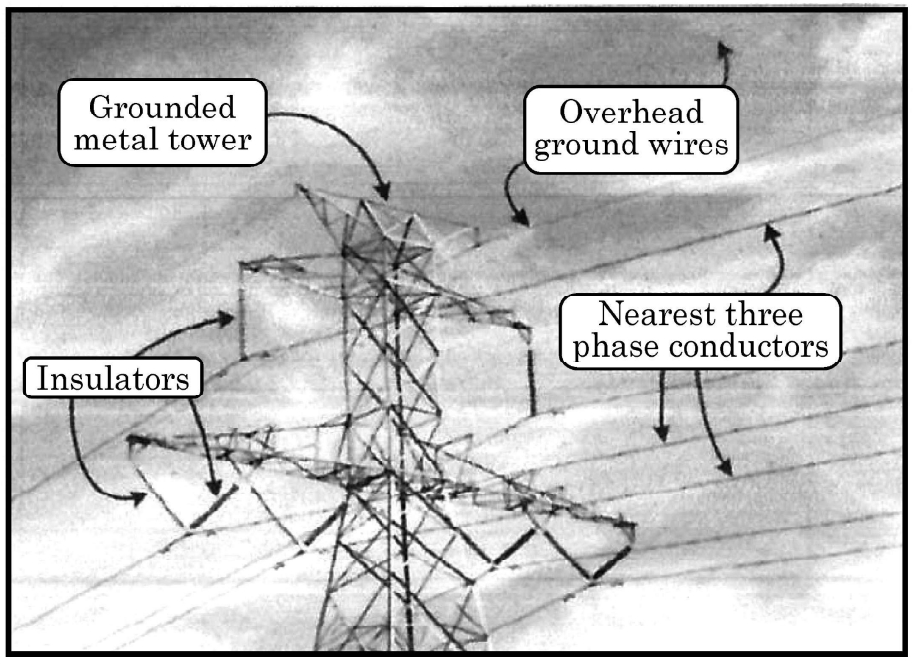
\includegraphics[width=\columnwidth]{figs/txn}
			\caption{Electrical transmission wires connected to a transmission tower.}
			\label{fig:txn1}
		\end{figure}
		Two such wires in the figure \ref{fig:txn1} lie along the following lines:
		\begin{align}
			l_1 &: \dfrac{x+1}{3}=\dfrac{y-3}{-2}=\dfrac{z+2}{-1}\\
			l_2 &: \dfrac{x}{-1}=\dfrac{y-7}{3}=\dfrac{z+7}{-2}
		\end{align}
		Based on the given information, answer the following questions:
		\begin{enumerate}
			\item	Are the $l_1$ and $l_2$ coplanar? Justify your answer.
			\item    Find the point of intersection of lines $l_1$ and $l_2$.
		\end{enumerate}

	\item Write the cartesian equation of the line PQ passing through points P$(2,2,1)$ and Q$(5,1,-2)$. Hence, find the y-coordinate of the point on the line PQ whose z-coordinate is -2.

	\item Find the distance between the lines $x=\dfrac{y-1}{2}=\dfrac{z-2}{3}$ and $x+1=\dfrac{y+2}{2}=\dfrac{z-1}{3}$.
	
	\item Find the shortest distance between the following lines:
		\begin{align}
			\vec{r}&=3\hat{i}+5\hat{j}+7\hat{k}+\lambda(\hat{i}-2\hat{j}+\hat{k})\\\vec{r}&=(-\hat{i}-\hat{j}-\hat{k})+\mu(7\hat{i}-6\hat{j}+\hat{k})
		\end{align}

	\item Two motorcycles A and B are running at a speed more than the allowed speed on the road (as shown in figure \ref{fig:bike1}) represented by the following lines 
		\begin{align}
			\vec{r}&=\lambda(\hat{i}+2\hat{j}-\hat{k})\\\vec{r}&=(3\hat{i}+3\hat{j})+\mu(2\hat{i}+\hat{j}+\hat{k})
		\end{align}
		\begin{figure}[H]
			\centering
			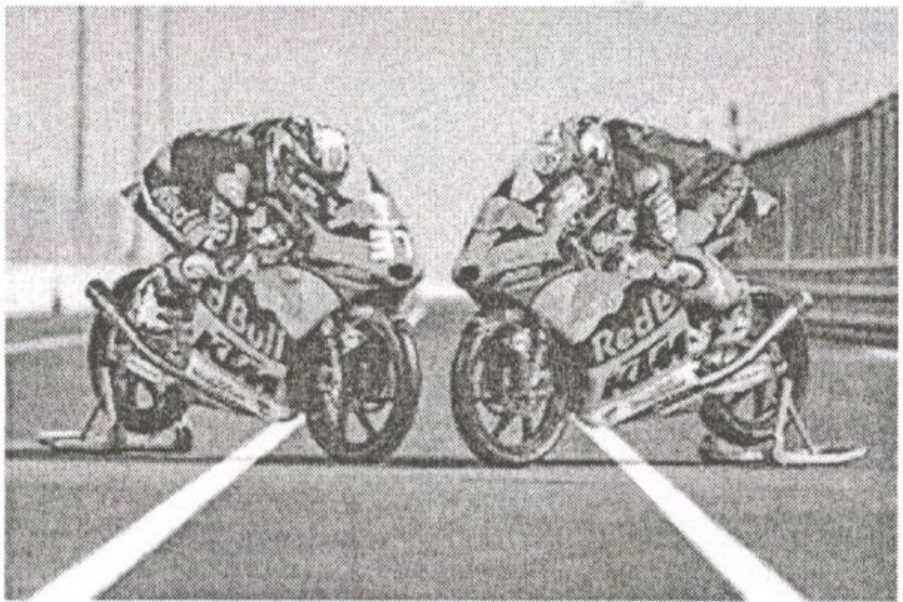
\includegraphics[width=\columnwidth]{figs/bike}
			\caption{Two motorcycles moving along the road in a straight line.}
			\label{fig:bike1}
		\end{figure}
		Based on the following information, answer the following questions:
		\begin{enumerate}
			\item Find the shortest distance between the given lines.
			\item Find a point at which the motorcycles may collide.
		\end{enumerate}
	
	\item Find the shortest distance between the following lines
		\begin{align}
			\vec{r}&=(\lambda+1)\hat{i}+(\lambda+4)\hat{j}-(\lambda-3)\hat{k}\\\vec{r}&=(3-\mu)\hat{i}+(2\mu+2)\hat{j}+(\mu+6)\hat{k}
		\end{align}
	
	\item Find the shortest distance between the following lines and hence write whether the lines are intersecting or not.
		\begin{align}
			\dfrac{x-1}{2}=\dfrac{y+1}{3}=z, \dfrac{x+1}{5}=\dfrac{y-2}{1}, z=2
		\end{align}

		\item Find the equation of the plane passing through the points $(2,1,0),(3,-2,-2)$ and $(1,1,7)$. Also, obtain its distance from the origin.

	\item The foot of a perpendicular drawn from the point $(-2,-1,-3)$ on a plane is $(1,-3,3)$. Find the equation of the plane.

	\item Find the cartesian and the vector equation of a plane which passes through the point $(3,2,0)$ and contains the line $\dfrac{x-3}{1}=\dfrac{y-6}{5}=\dfrac{z-4}{4}$.

	\item The distance between the planes $4x-4y+2z+5=0$ and $2x-2y+z+6=0$ is

		\begin{enumerate}

			\item $\dfrac{1}{6}$
			\item $\dfrac{7}{6}$
			\item $\dfrac{11}{6}$
			\item $\dfrac{16}{6}$
		\end{enumerate}

	\item Find the equation of the plane through the line of intersection of the planes
		\begin{align}
			\vec{r}\cdot(\hat{i}+3\hat{j})+6&=0\\\vec{r}\cdot(3\hat{i}-\hat{j}-4\hat{k})&=0
		\end{align}which is at a  unit distance from the origin.

		\item If the distance of the point $(1,1,1)$ from the plane $x-y+z+\lambda=0$ is $\dfrac{5}{\sqrt{3}}$, find the value(s) of $\lambda$.

	\item Find the distance of the point $(2,3,4)$ measured along the line $\dfrac{x-4}{3}=\dfrac{y+5}{6}=\dfrac{z+1}{2}$ from the plane $3x+2y+2z+5=0$.

	\item Find the distance of the point $P(4,3,2)$ from the plane determined by the points $A(-1,6,-5),B(-5,-2,3)$ and $C(2,4,-5)$.

	\item The distance of the line
		\begin{align}
		\vec{r}=(\hat{i}-\hat{j})+\lambda(\hat{i}+5\hat{j}+\hat{k})\end{align}
		from the plane
		\begin{align}
		\vec{r}\cdot(\hat{i}-\hat{j}+4\hat{k})=5\end{align}
		is
		\begin{enumerate}
			\item $\sqrt{2}$
			\item $\dfrac{1}{\sqrt{2}}$
			\item $\dfrac{1}{3\sqrt{2}}$
			\item $\dfrac{-2}{3\sqrt{2}}$
		\end{enumerate}

	\item Find a unit vector perpendicular to each of the vectors $(\vec{a}+\vec{b})$ and $(\vec{a}-\vec{b})$ where 
	\begin{align}
		\vec{a}&=\hat{i}+\hat{j}+\hat{k}\\\vec{b}&=\hat{i}+2\hat{j}+3\hat{k}
	\end{align}

	\item Find the distance of the point $(1,-2,9)$ from the point of intersection of the line
		\begin{align}
			\vec{r}=4\hat{i}+2\hat{j}+7\hat{k}+\lambda(3\hat{i}+4\hat{j}+2\hat{k})
		\end{align}and the plane
		\begin{align}
			\vec{r}\cdot(\hat{i}-\hat{j}+\hat{k})=10.
		\end{align}

	\item Find the area bounded by the curves $y=\abs{x-1}$ and $y=1$, using integration.

	\item Find the coordinates of the point where the line through $(4,-3,-4)$ and $(3,-2,2)$ crosses the plane $2x+y+z=6$.

	\item Fit a straight line trend by the method of least squares and find the trend value for the year 2008 using the data from Table \ref{tab:LC}:
		\begin{table}[H]
			\caption{Table showing yearly trend of production of goods in lakh tonnes \label{tab:LC}}
			%%%%%%%%%%%%%%%%%%%%%%%%%%%%%%%%%%%%%%%%%%%%%%%%%%%%%%%%%%%%%%%%%%%%%%
%%                                                                  %%
%%  This is the header of a LaTeX2e file exported from Gnumeric.    %%
%%                                                                  %%
%%  This file can be compiled as it stands or included in another   %%
%%  LaTeX document. The table is based on the longtable package so  %%
%%  the longtable options (headers, footers...) can be set in the   %%
%%  preamble section below (see PRAMBLE).                           %%
%%                                                                  %%
%%  To include the file in another, the following two lines must be %%
%%  in the including file:                                          %%
%%        \def\inputGnumericTable{}                                 %%
%%  at the beginning of the file and:                               %%
%%        \input{name-of-this-file.tex}                             %%
%%  where the table is to be placed. Note also that the including   %%
%%  file must use the following packages for the table to be        %%
%%  rendered correctly:                                             %%
%%    \usepackage[latin1]{inputenc}                                 %%
%%    \usepackage{color}                                            %%
%%    \usepackage{array}                                            %%
%%    \usepackage{longtable}                                        %%
%%    \usepackage{calc}                                             %%
%%    \usepackage{multirow}                                         %%
%%    \usepackage{hhline}                                           %%
%%    \usepackage{ifthen}                                           %%
%%  optionally (for landscape tables embedded in another document): %%
%%    \usepackage{lscape}                                           %%
%%                                                                  %%
%%%%%%%%%%%%%%%%%%%%%%%%%%%%%%%%%%%%%%%%%%%%%%%%%%%%%%%%%%%%%%%%%%%%%%



%%  This section checks if we are begin input into another file or  %%
%%  the file will be compiled alone. First use a macro taken from   %%
%%  the TeXbook ex 7.7 (suggestion of Han-Wen Nienhuys).            %%
\def\ifundefined#1{\expandafter\ifx\csname#1\endcsname\relax}


%%  Check for the \def token for inputed files. If it is not        %%
%%  defined, the file will be processed as a standalone and the     %%
%%  preamble will be used.                                          %%
\ifundefined{inputGnumericTable}

%%  We must be able to close or not the document at the end.        %%
 \def\gnumericTableEnd{\end{document}}


%%%%%%%%%%%%%%%%%%%%%%%%%%%%%%%%%%%%%%%%%%%%%%%%%%%%%%%%%%%%%%%%%%%%%%
%%                                                                  %%
%%  This is the PREAMBLE. Change these values to get the right      %%
%%  paper size and other niceties.                                  %%
%%                                                                  %%
%%%%%%%%%%%%%%%%%%%%%%%%%%%%%%%%%%%%%%%%%%%%%%%%%%%%%%%%%%%%%%%%%%%%%%

 \documentclass[12pt%
     %,landscape%
                    ]{report}
       \usepackage[latin1]{inputenc}
       \usepackage{fullpage}
       \usepackage{color}
       \usepackage{array}
       \usepackage{longtable}
       \usepackage{calc}
       \usepackage{multirow}
       \usepackage{hhline}
       \usepackage{ifthen}

 \begin{document}


%%  End of the preamble for the standalone. The next section is for %%
%%  documents which are included into other LaTeX2e files.          %%
\else

%%  We are not a stand alone document. For a regular table, we will %%
%%  have no preamble and only define the closing to mean nothing.   %%
    \def\gnumericTableEnd{}

%%  If we want landscape mode in an embedded document, comment out  %%
%%  the line above and uncomment the two below. The table will      %%
%%  begin on a new page and run in landscape mode.                  %%
%       \def\gnumericTableEnd{\end{landscape}}
%       \begin{landscape}


%%  End of theelse clause for this file being \input.              %%
\fi

%%%%%%%%%%%%%%%%%%%%%%%%%%%%%%%%%%%%%%%%%%%%%%%%%%%%%%%%%%%%%%%%%%%%%%
%%                                                                  %%
%%  The rest is the gnumeric table, except for the closing          %%
%%  statement. Changes below will alter the table's appearance.     %%
%%                                                                  %%
%%%%%%%%%%%%%%%%%%%%%%%%%%%%%%%%%%%%%%%%%%%%%%%%%%%%%%%%%%%%%%%%%%%%%%

\providecommand{\gnumericmathit}[1]{#1} 
%%  Uncomment the next line if you would like your numbers to be in %%
%%  italics if they are italizised in the gnumeric table.           %%
%\renewcommand{\gnumericmathit}[1]{\mathit{#1}}
\providecommand{\gnumericPB}[1]%
{\let\gnumericTemp=\\#1\let\\=\gnumericTemp\hspace{0pt}}
 \ifundefined{gnumericTableWidthDefined}
        \newlength{\gnumericTableWidth}
        \newlength{\gnumericTableWidthComplete}
        \newlength{\gnumericMultiRowLength}
        \global\def\gnumericTableWidthDefined{}
 \fi
%% The following setting protects this code from babel shorthands.  %%
 \ifthenelse{\isundefined{\languageshorthands}}{}{\languageshorthands{english}}
%%  The default table format retains the relative column widths of  %%
%%  gnumeric. They can easily be changed to c, r or l. In that case %%
%%  you may want to comment out the next line and uncomment the one %%
%%  thereafter                                                      %%
\providecommand\gnumbox{\makebox[0pt]}
%%\providecommand\gnumbox[1][]{\makebox}

%% to adjust positions in multirow situations                       %%
\setlength{\bigstrutjot}{\jot}
\setlength{\extrarowheight}{\doublerulesep}

%%  The \setlongtables command keeps column widths the same across  %%
%%  pages. Simply comment out next line for varying column widths.  %%
\setlongtables

\setlength\gnumericTableWidth{%
 53pt+%
 53pt+%
 106pt+%
0pt}
\def\gumericNumCols{3}
\setlength\gnumericTableWidthComplete{\gnumericTableWidth+%
         \tabcolsep*\gumericNumCols*2+\arrayrulewidth*\gumericNumCols}
\ifthenelse{\lengthtest{\gnumericTableWidthComplete > \linewidth}}%
         {\def\gnumericScale{\ratio{\linewidth-%
                        \tabcolsep*\gumericNumCols*2-%
                        \arrayrulewidth*\gumericNumCols}%
{\gnumericTableWidth}}}%
{\def\gnumericScale{1}}

%%%%%%%%%%%%%%%%%%%%%%%%%%%%%%%%%%%%%%%%%%%%%%%%%%%%%%%%%%%%%%%%%%%%%%
%%                                                                  %%
%% The following are the widths of the various columns. We are      %%
%% defining them here because then they are easier to change.       %%
%% Depending on the cell formats we may use them more than once.    %%
%%                                                                  %%
%%%%%%%%%%%%%%%%%%%%%%%%%%%%%%%%%%%%%%%%%%%%%%%%%%%%%%%%%%%%%%%%%%%%%%

\ifthenelse{\isundefined{\gnumericColA}}{\newlength{\gnumericColA}}{}\settowidth{\gnumericColA}{\begin{tabular}{@{}p{53pt*\gnumericScale}@{}}x\end{tabular}}
\ifthenelse{\isundefined{\gnumericColB}}{\newlength{\gnumericColB}}{}\settowidth{\gnumericColB}{\begin{tabular}{@{}p{150pt*\gnumericScale}@{}}x\end{tabular}}
\ifthenelse{\isundefined{\gnumericColC}}{\newlength{\gnumericColC}}{}\settowidth{\gnumericColC}{\begin{tabular}{@{}p{106pt*\gnumericScale}@{}}x\end{tabular}}

\begin{longtable}[c]{%
 b{\gnumericColA}%
 b{\gnumericColB}%
 b{\gnumericColC}%
 }

%%%%%%%%%%%%%%%%%%%%%%%%%%%%%%%%%%%%%%%%%%%%%%%%%%%%%%%%%%%%%%%%%%%%%%
%%  The longtable options. (Caption, headers... see Goosens, p.124) %%
% \caption{The Table Caption.}             \\ %
% \hline % Across the top of the table.
%%  The rest of these options are table rows which are placed on    %%
%%  the first, last or every page. Use \multicolumn if you want.    %%

%%  Header for the first page.                                      %%
% \multicolumn{3}{c}{The First Header} \\ \hline 
% \multicolumn{1}{c}{colTag} %Column 1
% &\multicolumn{1}{c}{colTag} %Column 2
% &\multicolumn{1}{c}{colTag} \\ \hline %Last column
% \endfirsthead

%%  The running header deinition.

%%
% \hline
% \multicolumn{3}{l}{\ldots\small\slshape continued} \\ \hline
% \multicolumn{1}{c}{colTag} %Column 1
% &\multicolumn{1}{c}{colTag} %Column 2
% &\multicolumn{1}{c}{colTag} \\ \hline %Last column
% \endhead

%%  The running footer definition.                                  %%
% \hline
% \multicolumn{3}{r}{\small\slshape continued\ldots} \\
% \endfoot

%%  The ending footer definition.                                   %%
% \multicolumn{3}{c}{That's all folks} \\ \hline 
% \endlastfoot
%%%%%%%%%%%%%%%%%%%%%%%%%%%%%%%%%%%%%%%%%%%%%%%%%%%%%%%%%%%%%%%%%%%%%%

\hhline{|-|-|-}
  \multicolumn{1}{|p{\gnumericColA}|}%
 {\gnumericPB{\raggedright}\gnumbox[l]{Year}}
 &\multicolumn{1}{p{\gnumericColB}|}%
	{\gnumericPB{\raggedright}\gnumbox[l]{Production (in lakh tonnes)}}
 %&\multicolumn{1}{p{\gnumericColC}|}%
 %{\gnumericPB{\raggedright}\gnumbox[l]{Description}}
\\
\hhline{|---|}
  \multicolumn{1}{|p{\gnumericColA}|}%
 {\gnumericPB{\raggedright}\gnumbox[l]{2001}}
 &\multicolumn{1}{p{\gnumericColB}|}%
 {\gnumericPB{\raggedright}\gnumbox[l]{30}}
 %&\multicolumn{1}{p{\gnumericColC}|}%
 %{\gnumericPB{\raggedright}\gnumbox[l]{Vertex A}}
\\
\hhline{|---|}
  \multicolumn{1}{|p{\gnumericColA}|}%
 {\gnumericPB{\raggedright}\gnumbox[l]{2002}}
 &\multicolumn{1}{p{\gnumericColB}|}%
 {\gnumericPB{\raggedright}\gnumbox[l]{35}}
 %&\multicolumn{1}{p{\gnumericColC}|}%
 %{\gnumericPB{\raggedright}\gnumbox[l]{Vertex B}}
\\
\hhline{|---|}
  \multicolumn{1}{|p{\gnumericColA}|}%
 {\gnumericPB{\raggedright}\gnumbox[l]{2003}}
 &\multicolumn{1}{p{\gnumericColB}|}%
 {\gnumericPB{\raggedright}\gnumbox[l]{36}}
 %&\multicolumn{1}{p{\gnumericColC}|}%
 %{\gnumericPB{\raggedright}\gnumbox[l]{Vertex C}}
\\
\hhline{|---|}
  \multicolumn{1}{|p{\gnumericColA}|}%
 {\gnumericPB{\raggedright}\gnumbox[l]{2004}}
 &\multicolumn{1}{p{\gnumericColB}|}%
 {\gnumericPB{\raggedright}\gnumbox[l]{32}}
 %&\multicolumn{1}{p{\gnumericColC}|}%
 %{\gnumericPB{\raggedright}\gnumbox[l]{Midpoint of AC}}
\\
\hhline{|---|}
  \multicolumn{1}{|p{\gnumericColA}|}%
 {\gnumericPB{\raggedright}\gnumbox[l]{2005}}
 &\multicolumn{1}{p{\gnumericColB}|}%
 {\gnumericPB{\raggedright}\gnumbox[l]{37}}
 %&\multicolumn{1}{p{\gnumericColC}|}%
 %{\gnumericPB{\raggedright}\gnumbox[l]{Midpoint of BC}}
\\
\hhline{|---|}
  \multicolumn{1}{|p{\gnumericColA}|}%
 {\gnumericPB{\raggedright}\gnumbox[l]{2006}}
 &\multicolumn{1}{p{\gnumericColB}|}%
 {\gnumericPB{\raggedright}\gnumbox[l]{40}}
 %&\multicolumn{1}{p{\gnumericColC}|}%
 %{\gnumericPB{\raggedright}\gnumbox[l]{Midpoint of AB}}
\\
\hhline{|-|-|-|}
\end{longtable}

\ifthenelse{\isundefined{\languageshorthands}}{}{\languageshorthands{\languagename}}
\gnumericTableEnd

		\end{table}
\end{enumerate}
